\chapter{Πειραματικά αποτελέσματα}
\section{Περιγραφή πειραμάτων}
Στόχος της παρούσας ενότητας είναι ο έλεγχος του συστήματος Automated Data Scientist, καθώς και της συνεισφοράς των τεχνικών που εφαρμόσαμε και περιγράψαμε στην ενότητα \ref{sec:techniques}. Προς αυτό το σκοπό σχεδιάσαμε τα ακόλουθα πειράματα, τα οποία θα αναλύσουμε στη συνέχεια:
\begin{itemize}
	\item αξιολόγηση των HPP μοντέλων
	\item αξιολόγηση του ensemble με προς-τα-εμπρός επιλογή μοντέλων
	\item συνολική αξιολόγηση του συστήματος
\end{itemize}

\paragraph{Περιγραφή σετ δεδομένων} Για τη διεξαγωγή των πειραμάτων συλλέξαμε ένα πλήθος 123 σετ δεδομένων από διάφορες πηγές. (Στο παράρτημα \ref{appendix:Datasets} βρίσκεται ένας λεπτομερής κατάλογος περιγραφής τους.) Άξονας αναζήτησης κατά τη συλλογή ήταν η εύρεση σετ δεδομένων δυαδικής ταξινόμησης με ετερογενή χαρακτηριστικά, ώστε ο έλεγχος του συστήματος να είναι αντιπροσωπευτικός για το πραγματικό πλήθος σετ δεδομένων. Προκειμένου να υπάρχει μία κοινή διεπαφή για τα πειράματα ήταν απαραίτητος ο "καθαρισμός" των σετ δεδομένων μέσω των ακόλουθων βημάτων:
\begin{itemize}
	\item μετατροπή αρχείων σε comma-delimited .csv. Τα πηγαία αρχεία βρίσκονταν σε μορφές .csv, .txt, .xlsx, .arff και .mysql.
	\item καθορισμός κλάσης. Στη πλειοψηφία των περιπτώσεων η κλάση αναγνωριζόταν χειροκίνητα από την περιγραφή του σετ δεδομένων. Συλλέχθηκαν και σετ δεδομένων που ήταν πολλαπλής ταξινόμησης και παλινδρόμησης. Στην πρώτη περίπτωση έγινε αντιστοίχηση σε δύο ουσιώδεις κλάσεις, ενώ στη δεύτερη βρέθηκε η μέση τιμή της μεταβλητής κλάσης και χρησιμοποιήθηκε ως κατώφλι για το διαχωρισμό των παραδειγμάτων σε δύο κλάσεις.
	\item αναγνώριση άγνωστων τιμών. Στα αρχεία που περιείχαν άγνωστες τιμές χρησιμοποιούνταν διάφοροι συμβολισμοί ("?", "*", "") οι οποίοι αντικαταστάθηκαν από κενά, ώστε να αναγνωρίζονται από την R ως NAs (Not Available).  
\end{itemize}
\section{Αξιολόγηση της τεχνικής βελτιστοποίησης υπερ-παραμέτρων με μετα-μάθηση και χρήση διαστημάτων πρόβλεψης}
Όπως είδαμε στην ενότητα \ref{sec:HPP} προϊόντα αυτής της τεχνικής είναι τα HPP μοντέλα, καθένα εκ των οποίων έχει εκπαιδευτεί στη πρόβλεψη μίας υπερ-παραμέτρου ενός αλγορίθμου μηχανικής μάθησης. Σε αυτό το σημείο θα αξιολογήσουμε τα μοντέλα αυτά ως προς το σκοπό τους, δηλαδή πόσο καλά προβλέπουν τις βελτιστοποιημένες υπερ-παραμέτρους. Επίσης, θα σχολιάσουμε τη συνεισφορά της χρήσης διαστημάτων πρόβλεψης.

Για την παραγωγή των σετ μετα-δεδομένων, τα οποία χρησιμοποιούνται για την εκπαίδευση των HPP μοντέλων, είναι απαραίτητα δύο στάδια:
\begin{itemize}
	\item Εξαγωγή των μετα-χαρακτηριστικών κάθε σετ δεδομένων. Τα μετα-χαρακτηριστικά που χρησιμοποιήσαμε περιγράφονται στον Πίνακα \ref{table:meta}, υπολογίστηκαν με χρήση του πακέτου mf\-Extractor του συστήματός μας και βασίστηκαν στη δουλειά της ομάδας που υλοποίησε το λογισμικό autosklearn. Καθώς τα μετα-χαρακτηριστικά που επιλέξαμε αφορούν μόνο μη-κατηγορικά χαρακτηριστικά, πριν τον υπολογισμό τους έγινε μετατροπή των κατηγορικών χαρακτηριστικών σε μεταβλητές-δείκτες. 
	 \begin{table}[!htb]
	 	\begin{center}
	 	\caption{Λίστα μετα-χαρακτηριστικών, τα οποία χρησιμοποιήθηκαν για την εκπαίδευση των HPP μοντέλων}
	 	\label{table:meta}
	 		\begin{tabular}{ |c| } 
	 			\hline
	 			Μετα-χαρακτηριστικά\\
	 			\hline
	 			Κλάσμα χαρακτηριστικών για 95$\%$ διακύμανση των PCA \\ 
	 			Κυρτότητα πρώτης PCA συνιστώσας   \\ 
	 			Ασσυμετρία πρώτης PCA συνιστώσας   \\ 
	 			Ελάχιστη ασυμμετρία \\
	 			Μέγιστη ασυμμετρία \\
	 			Μέση τιμή ασυμμετρίας \\
	 			Τυπική απόκλιση ασυμμετρίας \\
	 			Ελάχιστη κυρτότητα \\
	 			Μέγιστη κυρτότητα \\
	 			Μέση τιμή κυρτότητας \\
	 			Τυπική απόκλιση κυρτότητας \\        	
	 			\hline
	 		\end{tabular}    
	 	\end{center}
	 \end{table}
	\item Εύρεση των βέλτιστων υπερ-παραμέτρων για κάθε αλγόριθμο. Προς αυτό ο σκοπό χρησιμοποιήθηκε η βιβλιοθήκη HPOlib, την οποία έχουμε περιγράψει στην Eνότητα \ref{section:tools}. Ο αλγόριθμος που επιλέχθηκε ήταν ο Tree Parzen Estimator, καθώς είναι σημαντικά ταχύτερος από τους υπόλοιπους. Από τη πλευρά μας ήταν απαραίτητος ο ορισμός του χώρου αναζήτησης υπερ-παραμέτρων και της συνάρτησης κόστους για κάθε αλγόριθμο, η οποία ορίστηκε ως $ Cost = 1- Accuracy$. Στον Πίνακα \ref{table:algorithms} μπορούμε να δούμε τους αλγορίθμους μάθησης με τους οποίους ασχοληθήκαμε, καθώς και τις υπερπαραμέτρους τους.

\end{itemize}
	\begin{table}[!htb]
		\begin{center}
				\caption[Οι αλγόριθμοι που χρησιμοποιεί το σύστημα Automated Data Scientist και οι υπερ-παράμετροί του]{Οι αλγόριθμοι που χρησιμοποιεί το σύστημα Automated Data Scientist και οι υπερ-παράμετροί τους, όπως τις ορίζει το πακέτο caret. knn: κ-κοντινότερος γείτονας, rpart: δέντρο ταξινόμησης και παλινδρόμησης (CART), nnet: \gls{ΤΝΝ}, svmRadial: \gls{SVM} με χρήση γκαουσιανού πυρήνα, nb: Naive Bayes.} \label{table:meta}
			\begin{tabular}{ |c|c|c|c|c| } 
				\hline
				knn & rpart & nnet & svmRadial & nb\\
				\hline
			    k & cp & size& C & fL\\
			     &  & decay& sigma & usekernel \\
			     &  &    & & adjust \\
				\hline
			\end{tabular}    
		\end{center}
		\label{table:algorithms}
	\end{table} 
	
Στα πειράματα που ακολουθούν έχουμε χρησιμοποιήσει τη τεχνική Leave one out για την αξιολόγηση των μοντέλων, 10-fold cross-validation για τη ρύθμιση και ως κριτήριο της απόδοσης των μοντέλων παλινδρόμησης τη ρίζα του μέσου τετραγωνικού σφάλματος (root mean squared error).
\begin{figure}[H]
\begin{minipage}{0.48\textwidth}
		\noindent
		\begin{center}
				\captionof{table}{Επιλογή αλγορίθμου για την υπερ-παράμετρο C του SVM}
				\begin{tabular}{ |c|c|c|c| } 
					\hline
					& lm & lm+BoxCox & svmRadial\\
					\hline
					rmse & & &\\
					\hline
					Rsquared & & & \\
					\hline 
					p-value & & &\\				
					\hline
				\end{tabular}   
		\end{center}
\end{minipage} \qquad
\begin{minipage}{0.48\textwidth}
		\centering
          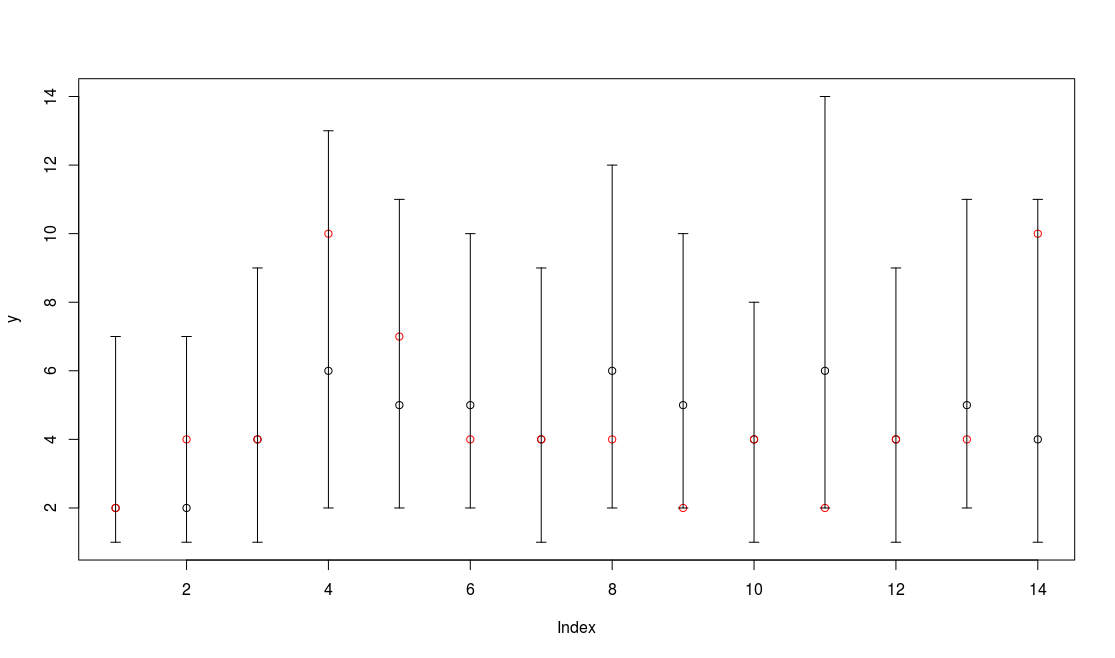
\includegraphics[width=\textwidth]{intervals}
		\caption{Διάστηματα πρόβλεψης για την υπερ-παράμετρο sigma του SVM.}	
\end{minipage}
\begin{minipage}{0.48\textwidth}
	\noindent
	\begin{center}
		\captionof{table}{Επιλογή αλγορίθμου για την υπερ-παράμετρο cp του rpart}
		\begin{tabular}{ |c|c|c|c| } 
			\hline
			& lm & lm+BoxCox & svmRadial\\
			\hline
			rmse & & &\\
			\hline
			Rsquared & & & \\
			\hline 
			p-value & & &\\				
			\hline
		\end{tabular}   
	\end{center}
\end{minipage} \qquad
\begin{minipage}{0.48\textwidth}
	 	\centering
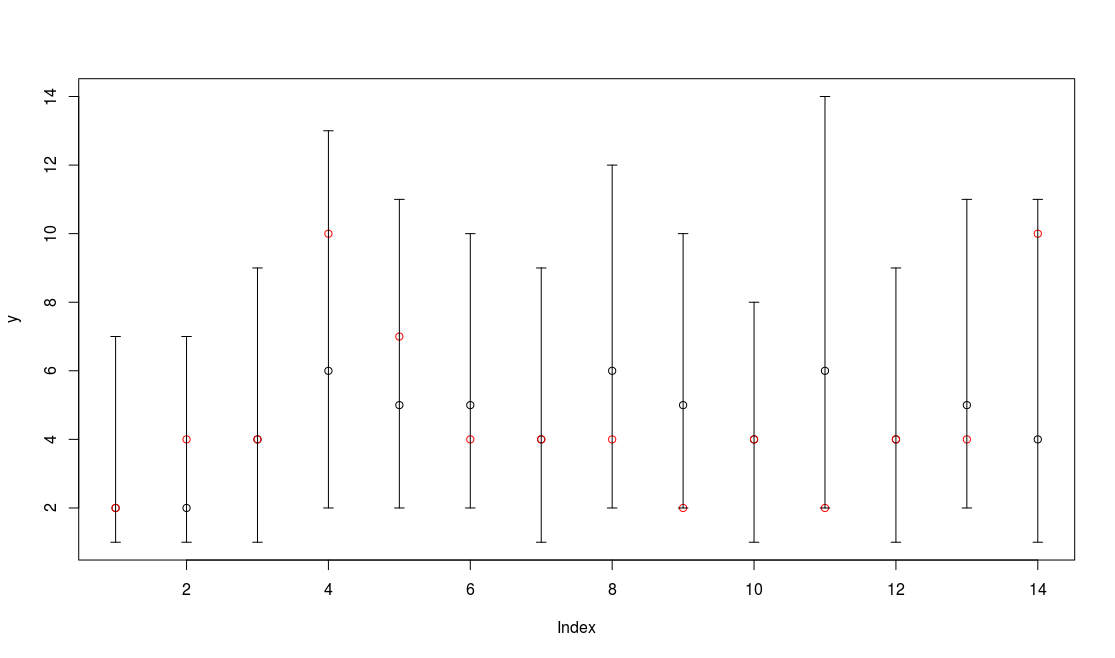
\includegraphics[width=0.9\textwidth]{intervals}
	 	\caption{Διάστηματα πρόβλεψης για την υπερ-παράμετρο cp του rpart.}	
\end{minipage}
\begin{minipage}{0.48\textwidth}
	\noindent
	\begin{center}
		\captionof{table}{Επιλογή αλγορίθμου για την υπερ-παράμετρο decay του nnet}
		\begin{tabular}{ |c|c|c|c| } 
			\hline
			& lm & lm+BoxCox & svmRadial\\
			\hline
			rmse & & &\\
			\hline
			Rsquared & & & \\
			\hline 
			p-value & & &\\				
			\hline
		\end{tabular}   
	\end{center}
\end{minipage} \qquad
\begin{minipage}{0.48\textwidth}
	\centering
	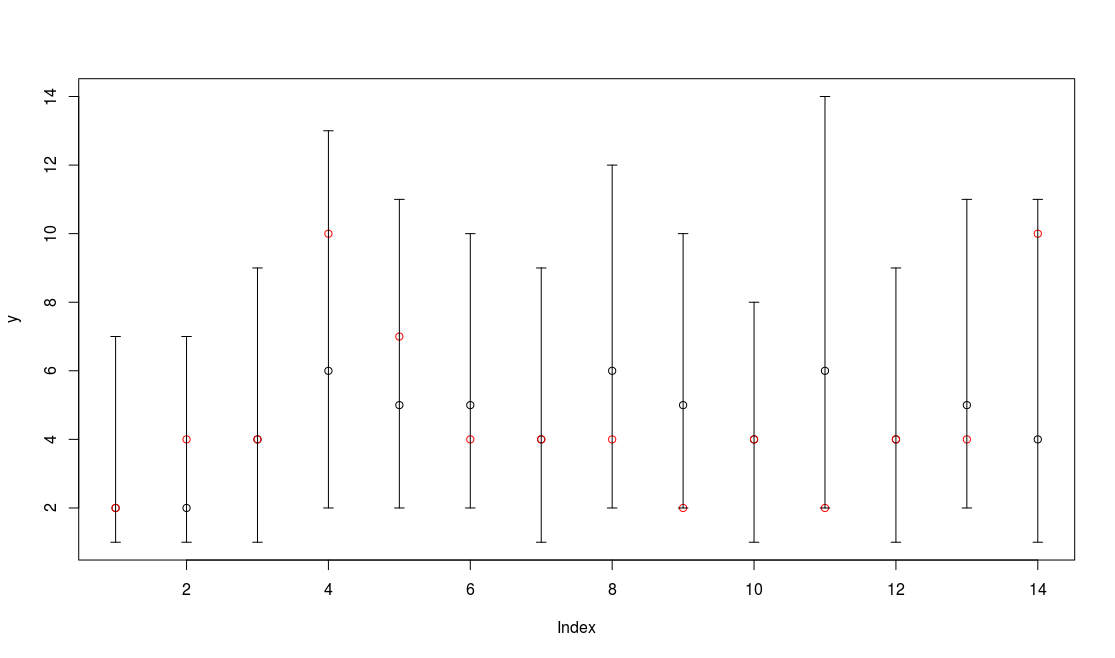
\includegraphics[width=\textwidth]{intervals}
	\caption{Διάστηματα πρόβλεψης για την υπερ-παράμετρο decay του nnet.}	
\end{minipage}
\begin{minipage}{0.48\textwidth}
	\noindent
	\begin{center}
		\captionof{table}{Επιλογή αλγορίθμου για την υπερ-παράμετρο size του nnet}
		\begin{tabular}{ |c|c|c|c| } 
			\hline
			& lm & lm+BoxCox & svmRadial\\
			\hline
			rmse & & &\\
			\hline
			Rsquared & & & \\
			\hline 
			p-value & & &\\				
			\hline
		\end{tabular}   
	\end{center}
\end{minipage} \qquad
\begin{minipage}{0.48\textwidth}
	\centering
	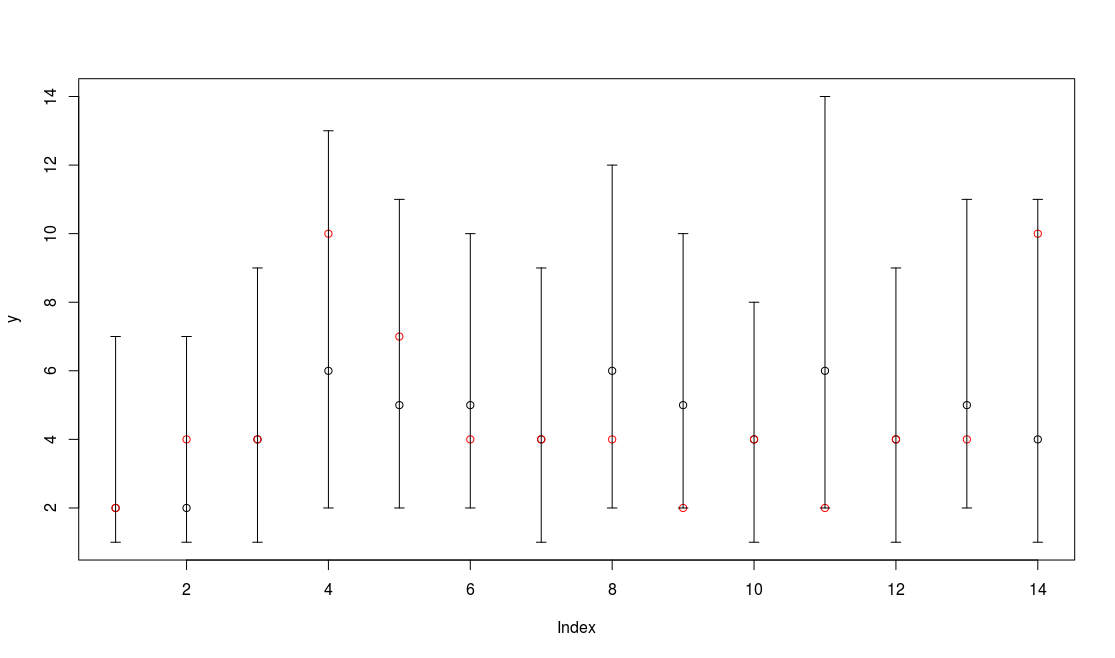
\includegraphics[width=\textwidth]{intervals}
	\caption{Διάστηματα πρόβλεψης για την υπερ-παράμετρο size του nnet.}	
\end{minipage}
\begin{minipage}{0.48\textwidth}
	\noindent
	\begin{center}
		\captionof{table}{Επιλογή αλγορίθμου για την υπερ-παράμετρο fL του nb}
		\begin{tabular}{ |c|c|c|c| } 
			\hline
			& lm & lm+BoxCox & svmRadial\\
			\hline
			rmse & & &\\
			\hline
			Rsquared & & & \\
			\hline 
			p-value & & &\\				
			\hline
		\end{tabular}   
	\end{center}
\end{minipage} \qquad
\begin{minipage}{0.48\textwidth}
	\centering
	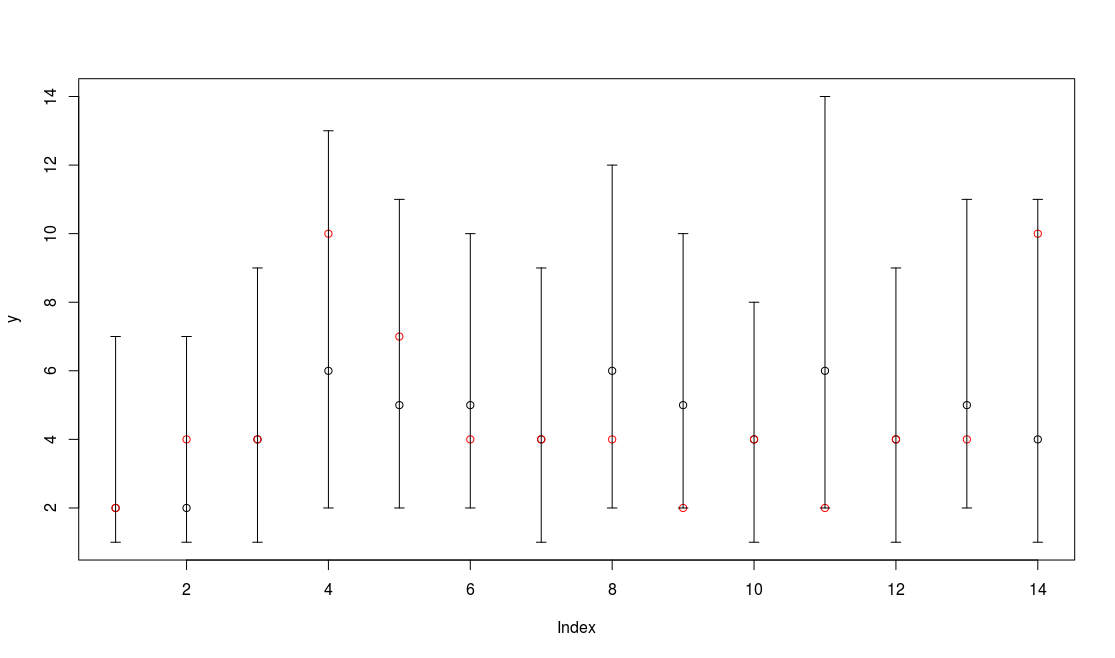
\includegraphics[width=\textwidth]{intervals}
	\caption{Διάστηματα πρόβλεψης για την υπερ-παράμετρο fL του nb.}	
\end{minipage}
\begin{minipage}{0.48\textwidth}
	\noindent
	\begin{center}
		\captionof{table}{Επιλογή αλγορίθμου για την υπερ-παράμετρο usekerne του nb}
		\begin{tabular}{ |c|c|c|c| } 
			\hline
			& lm & lm+BoxCox & svmRadial\\
			\hline
			rmse & & &\\
			\hline
			Rsquared & & & \\
			\hline 
			p-value & & &\\				
			\hline
		\end{tabular}   
	\end{center}
\end{minipage} \qquad
\begin{minipage}{0.48\textwidth}
	\centering
	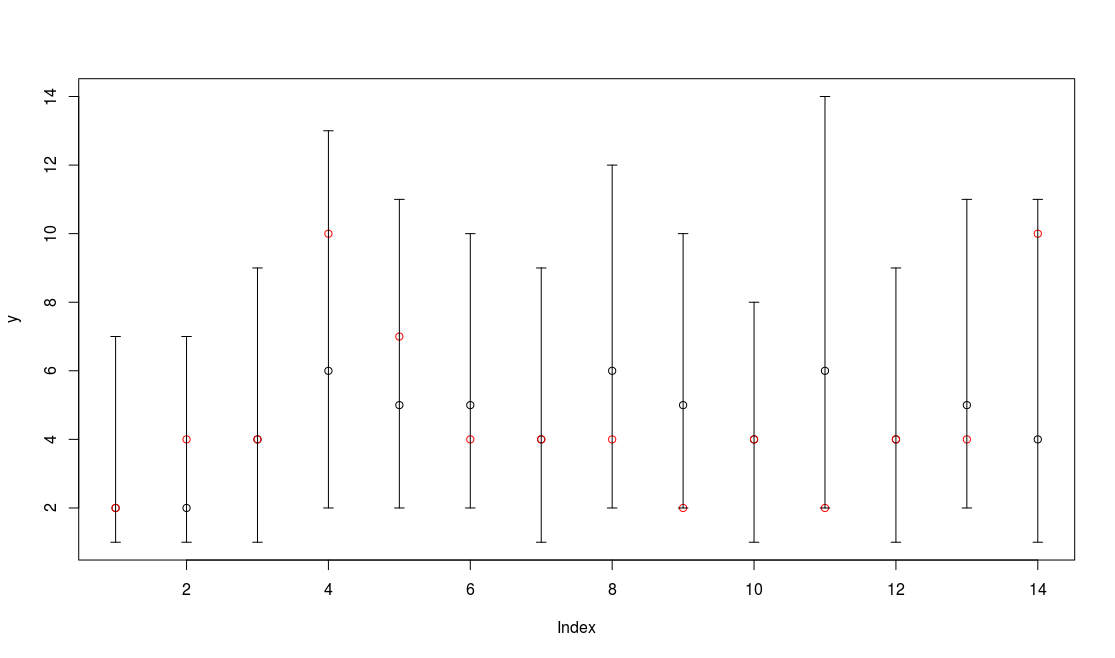
\includegraphics[width=\textwidth]{intervals}
	\caption{Καμπύλη ROC  για την υπερ-παράμετρο usekernel του nb.}	
\end{minipage}
\begin{minipage}{0.48\textwidth}
	\noindent
	\begin{center}
		\captionof{table}{Επιλογή αλγορίθμου για την υπερ-παράμετρο adjust του nb.}
		\begin{tabular}{ |c|c|c|c| } 
			\hline
			& lm & lm+BoxCox & svmRadial\\
			\hline
			rmse & & &\\
			\hline
			Rsquared & & & \\
			\hline 
			p-value & & &\\				
			\hline
		\end{tabular}   
	\end{center}
\end{minipage} \qquad
\begin{minipage}{0.48\textwidth}
	\centering
	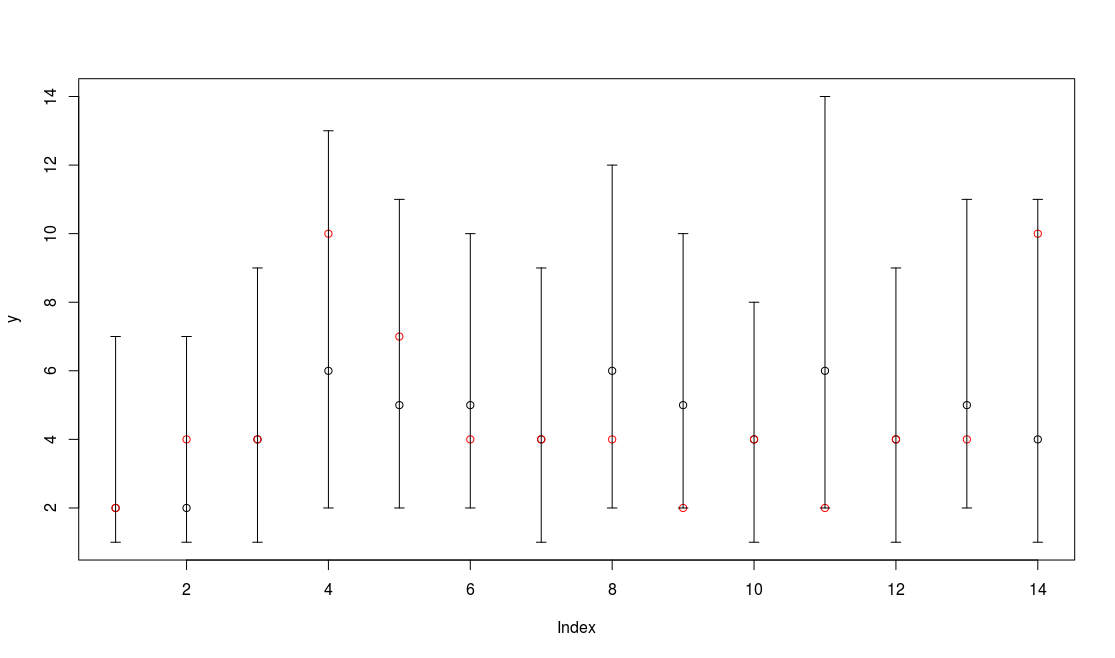
\includegraphics[width=\textwidth]{intervals}
	\caption{Διάστηματα πρόβλεψης για την υπερ-παράμετρο adjust του nb.}	
\end{minipage}
\end{figure}

\FloatBarrier

\paragraph{Συμπεράσματα}
Τα μοντέλα HPP που εκπαιδεύσαμε απέχουν κατά πολύ από το να προβλέπουν επακριβώς τις υπερ-παραμέτρους. Το γεγονός αυτό μάλλον οφείλεται στα μετα-χαρακτη\-ρι\-στικά και συγκεκριμένα την αδυναμία τους να περιγράψουν τις συναρτήσεις-στόχους που θέσαμε. Είναι γεγονός πως δεν είμαστε βέβαιοι για την επιτευξιμότητα της πρόβλεψης υπερ-παραμέτρων, τα πειράματά μας ωστόσο δεν απορρίπτουν την ύπαρξη κάποια συσχέτισης μεταξύ αυτών και των μετα-χαρακτηριστικών.

Η προσθήκη των διαστημάτων πρόβλεψης αποδεικνύεται ότι αναιρεί την αδυναμία των μοντέλων HPP, καθώς η βέλτιστη τιμή βρίσκεται σχεδόν πάντα μέσα στο διάστημα πρόβλεψης, προσδίδοντας βαρύτητα στην αξιολόγηση του ensemble, η οποία ακολουθεί.  
\section{Αξιολόγηση της τεχνικής σχηματισμού ensemble με προς τα εμπρός επιλογή μοντέλων} \label{section:tensemble}
H αξιολόγηση της τεχνικής ensemble που χρησιμοποιήσαμε επιχειρεί να επιβεβαιώσει δύο προσδοκίες:
\begin{itemize}
	\item Ο ensemble παρουσιάζει τουλάχιστον το ίδιο καλή απόδοση με το καλύτερο μοντέλο, το οποίο βρίσκεται στην αποθήκη βελτιστοποιημένων μοντέλων. Προς αυτό το σκοπό θα συγκρίνουμε την απόδοση του ensemble με αυτήν του εκάστοτε βέλτιστου μοντέλου με δύο τεχνικές: στατιστικά τεστ υπόθεσης και διαγράμματα προφίλ απόδοσης.
	\item Ο ensemble προσθέτει μοντέλα με το βέλτιστο τρόπο. Ουσιαστικά θέλουμε να επιβεβαιώσουμε τη σωστή λειτουργία του ensemble, δηλαδή ότι σε κάθε επανάληψη έχουμε είτε σταθερή είτε βελτιωμένη απόδοση.
\end{itemize}

Για τα πειράματά μας εκπαιδεύουμε τα μοντέλα στο $80\%$ των σετ δεδομένων και κρατάμε τα υπόλοιπα για την αξιολόγηση του ensemble, η οποία γίνεται ως εξής: εξάγονται τα μετα-χαρακτηριστικά των σετ δεδομένων, προβλέπονται οι βέλτιστες υπερ-παράμετροι για κάθε αλγόριθμο μάθησης, εκπαιδεύονται τα μοντέλα και τέλος σχηματίζεται ο ensemble. Για κάθε σετ δεδομένων καταγράφεται η απόδοση του ensemble και του βέλτιστου μοντέλου ως η ακρίβεια (accuracy) που επιτεύχθηκε με 10-fold cross-validation. 

Εφαρμόζωντας το Wilcoxon-rank sum τεστ με επίπεδο εμπιστοσύνης $95\%$ διαπιστώνουμε πως ..., καθώς το p-value ισούται με ... .

\paragraph{Διαγράμματα προφίλ απόδοσης} 	Τα διαγράμματα προφίλ απόδοσης (performance profile plots) \citep{Dolan2002} αποτελούν ένα εργαλείο αξιολόγησης και σύγκρισης της απόδοσης εργαλείων βελτιστοποίησης. Χρησιμοποιούνται σε περιπτώσεις εφαρμογής διαφορετικών τεχνικών βελτιστοποίησης σε ένα σύνολο προβλημάτων ως εναλλακτική απεικόνιση εκτενών πινάκων, μιας συνηθισμένης και προβληματικής λύσης. Το προφίλ απόδοσης είναι η αθροιστική συνάρτηση κατανομής μιας τεχνικής για μία μετρική απόδοσης.

Ως μετρική απόδοσης ορίζουμε το λόγο της απόδοσης της τρέχουσας τεχνικής προς τη μεγαλύτερη απόδοση που επιτεύχθηκε από οποιαδήποτε τεχνική για ένα συγκεκριμένο σετ δεδομένων, δηλαδή

\begin{equation}
r_{p,s}= \frac{t_{p,s}}{\max\{{t_{p,s} : s \in S}\}}    
\end{equation} 

όπου r ο λόγος απόδοσης, t η ακρίβεια, p το σετ δεδομένων και s η τεχνική.

Το διάγραμμα απεικονίζει τη τιμή
\begin{equation}
\rho_{\tau}= \frac{size\{{p \in P : r_{p,s} \leq \tau  }\}}{n_p}   
\end{equation}

όπου $n_p$ το πλήθος των σετ δεδομένων. Η τιμή αυτή εκφράζει την πιθανότητα μία τεχνική να βρίσκεται σε απόσταση $\tau$ από τον καλύτερο λόγο απόδοσης.  Επομένως το σημείο $\tau = 1$ εκφράζει τη πιθανότητα μία τεχνική να είναι η βέλτιστη.


\begin{figure}[!htb]
	\begin{center}
		\caption[Διάγραμμα προφίλ απόδοσης για τη σύγκριση του ensemble με το βέλτιστο μοντέλο]{Διάγραμμα προφίλ απόδοσης για τη σύγκριση του ensemble με το βέλτιστο μοντέλο: Παρατηρούμε πως }
	\end{center}
\end{figure}

\begin{figure}[!htb]
	\begin{center}
		\caption[Διάγραμμα εξέλιξης ensemble για το σετ δεδομένων (όνομα)]{Διάγραμμα εξέλιξης ensemble για το σετ δεδομένων (όνομα): Παρατηρούμε πως σε κάθε επανάληψη η απόδοση του ensemble είτε μειώνεται είτε παραμένει σταθερή. }
	\end{center}
\end{figure} 	

\paragraph{Συμπεράσματα}
\section{Αξιολόγηση συστήματος Automated Data Scientist}\label{section:eval_system}
Η αξιολόγηση του Automated Data Scientist στοχεύει να αποδείξει ότι το σύστημα που έχουμε σχεδιάσει έχει απόδοση συγκρίσιμη με τεχνικές της σύγχρονης βιβλιογραφίας. Καθώς η ουσιαστική πρωτοτυπία του συστήματος βρίσκεται στον τρόπο με τον οποίο γίνεται η βελτιστοποίηση των υπερ-παρα\-μέ\-τρων για τα μοντέλα μηχανικής μάθησης που χρησιμοποιούμε θα συγκρίνουμε το σύστημά μας με δύο τεχνικές βελτιστοποίησης:
\begin{itemize}
	\item πλεγματική αναζήτηση. Πρόκειται για τη συνηθέστερη τεχνική αναζήτησης υπερ\-παραμέτρων μέχρι και σήμερα.
	\item Tree Parzen Estimator. Η τεχνική αυτή, που έχει περιγραφεί στην ενότητα \ref{section:SMBO} αποτελεί state of the art στο χώρο του AutoML.
\end{itemize}

Η διεξαγωγή των πειραμάτων ακολουθεί τη λογική της ενότητας \ref{section:tensemble}. Έχουμε πραγματοποιήσει 6 διαφορετικά πειράματα: ένα για το συνολικό σύστημα και ένα χρησιμοποιώντας στον ensemble μοντέλα μόνο ενός αλγορίθμου μάθησης. Οι υποπεριπτώσεις αυτές λαμβάνονται υπόψη για τη σύγκριση των τριών τεχνικών επί ίσοις όροις. Φυσικά εμείς ενδιαφερόμαστε περισσότερο για την απόδειξη υπεροχής του συνολικού συστήματος.  

[Ακολουθούν τα διαγράμματα προφίλ απόδοσης]
	
\paragraph{Συμπεράσματα}